\documentclass[11pt]{article}
\usepackage[margin=1in]{geometry}
\usepackage{graphicx}
\usepackage{amsmath, amssymb}
\usepackage{hyperref}
\usepackage{bookmark}
\usepackage{titlesec}
\usepackage{fancyhdr}
\usepackage{listings}
\usepackage{xcolor}
\usepackage{float}
\usepackage{arydshln}
\usepackage{indentfirst}
\usepackage{multicol}
\usepackage{subcaption}
\usepackage{physics}
\usepackage{csvsimple}
\usepackage{lipsum}

% For removing reference section title, we will add it manually later on.
\renewcommand{\refname}{}

% Setup for hyperlinks, for pretty URL's.
\hypersetup{
    colorlinks=true,
    linkcolor=blue,
    filecolor=magenta,      
    urlcolor=cyan,
}

% Listings settings for MATLAB, for pretty code.
\lstset{
  language=Matlab,
  basicstyle=\footnotesize\ttfamily,
  breaklines=true,
  keywordstyle=\color{blue},
  numbers=left,
  numberstyle=\tiny\color{gray},
  stringstyle=\color{purple},
  commentstyle=\color{teal},
  morecomment=[l][\color{magenta}]{\#},
  frame=single,
  rulecolor=\color{black},
  showstringspaces=false,
  tabsize=2,
  title=\lstname % Show the filename of files included with \lstinputlisting;
}


% Title formatting, so you will not need to abuse "commands" to make it work.
\titleformat*{\section}{\large\bfseries}
\titleformat*{\subsection}{\normalsize\bfseries}
\titleformat*{\subsubsection}{\small\bfseries}

% Prevent section numbers
\setcounter{secnumdepth}{0}

\begin{document}

\textbf{Name/Surname:} John Doe \hfill \textbf{Date:} DD.MM.YYYY % Use Day.Month.Year standard

\textbf{Student ID:} xxxxxxx \hfill \textbf{Signature:}
    \includegraphics[width=0.02\linewidth]{image.png} % Add your signature, use filename "image.png"!


\textbf{Section:} CHANGE THIS TO YOUR SECTION

\begin{center}
  \textbf{Experiment X and Y: Name of X \& Name of Y}
\end{center}

\section{Abstract}
% Brief summary of both experiments and main findings.


\section{Introduction \& Background/Theory}
% Introduce both experiments and their theoretical backgrounds.
% Explain the model and its underpinnings for both experiments.

% An equation example.
\begin{equation}
    E_x=-\frac{dV}{dx}
    \label{eq:eqtoef}
\end{equation}

\section{Description of Experiment and Method(s)}
\subsection{Experiment X: Name of X}
% Description of Experiment X setup and methodology.

% Example to use multicols.
\begin{multicols}{2}

  % Just a generic text, remove it while writing a report.
  \lipsum[1]

  \columnbreak
% Example of figure environment usage with includegraphics
\begin{figure}[H]
    \centering
    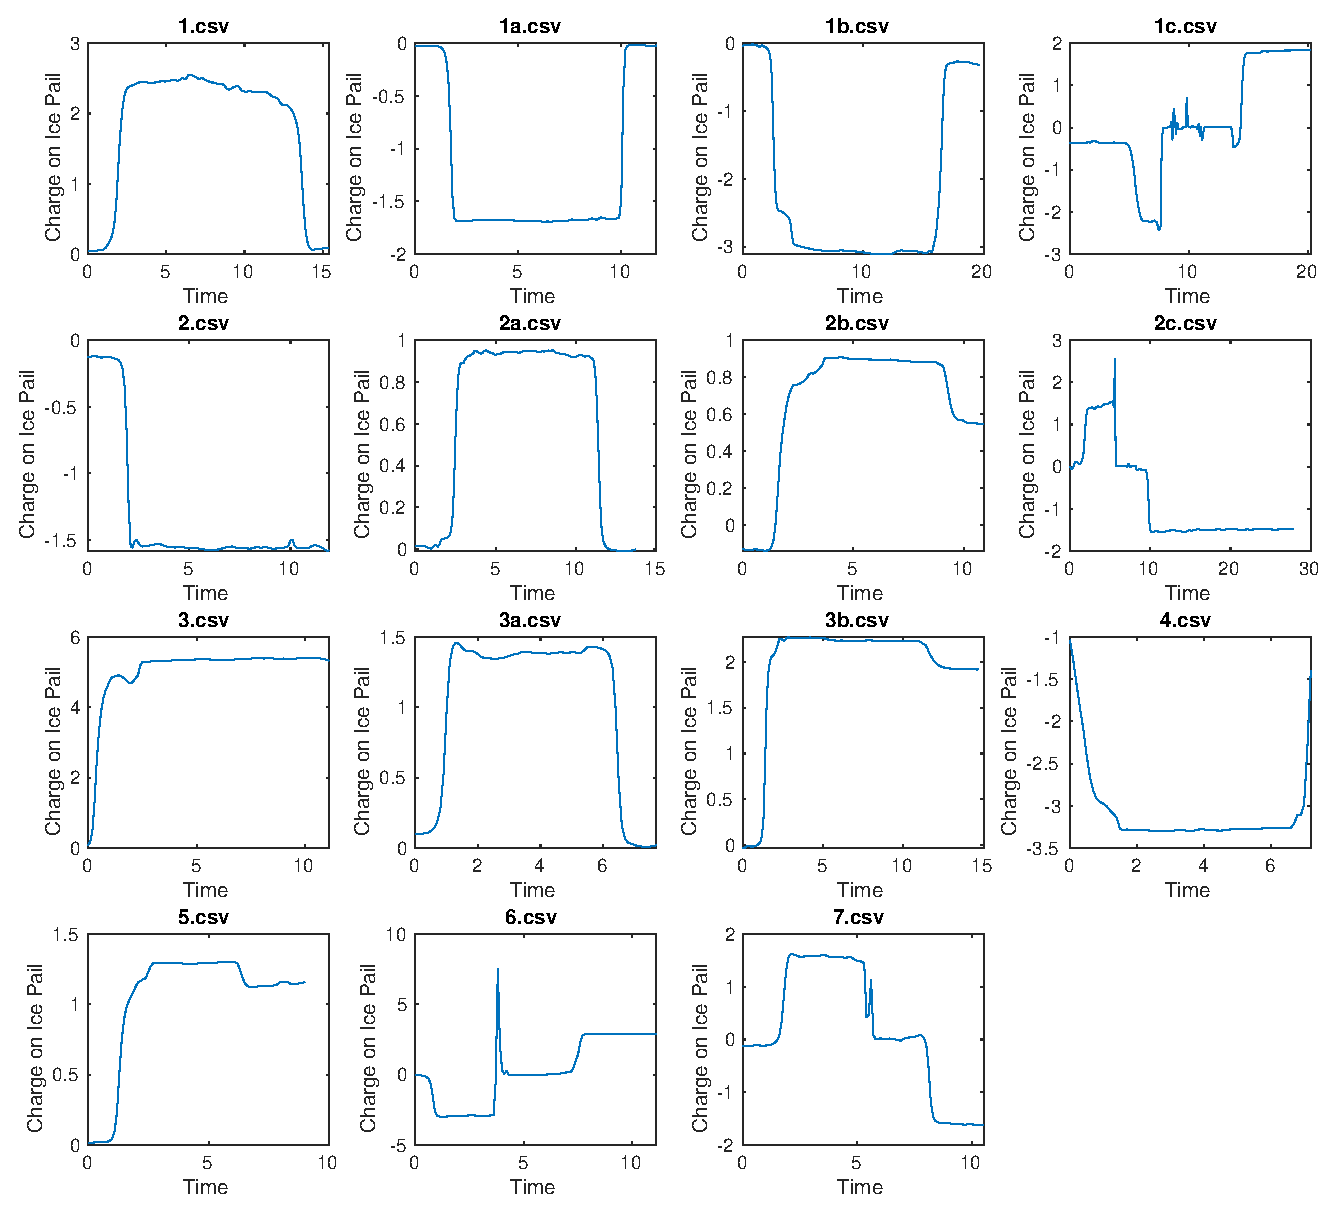
\includegraphics[width=0.5\linewidth]{figure1.eps}
    \caption{Setup for experiment 1.}
    \label{fig:setupexp1}
\end{figure}
\end{multicols}

\subsection{Experiment Y: Name of Y    }
% Description of Experiment Y setup and methodology.


\section{Results \& Discussion}
\subsection{Experiment X: Name of X}
% Results and discussion for Experiment X.

% Example of referring to a Figure, can also be used with table environment.
Figure~\ref{fig:exp1data}

% Example of EPS file import. You can use other file types as well. Remember, \includegraphics only works on images.
\begin{figure}[H]
\centering
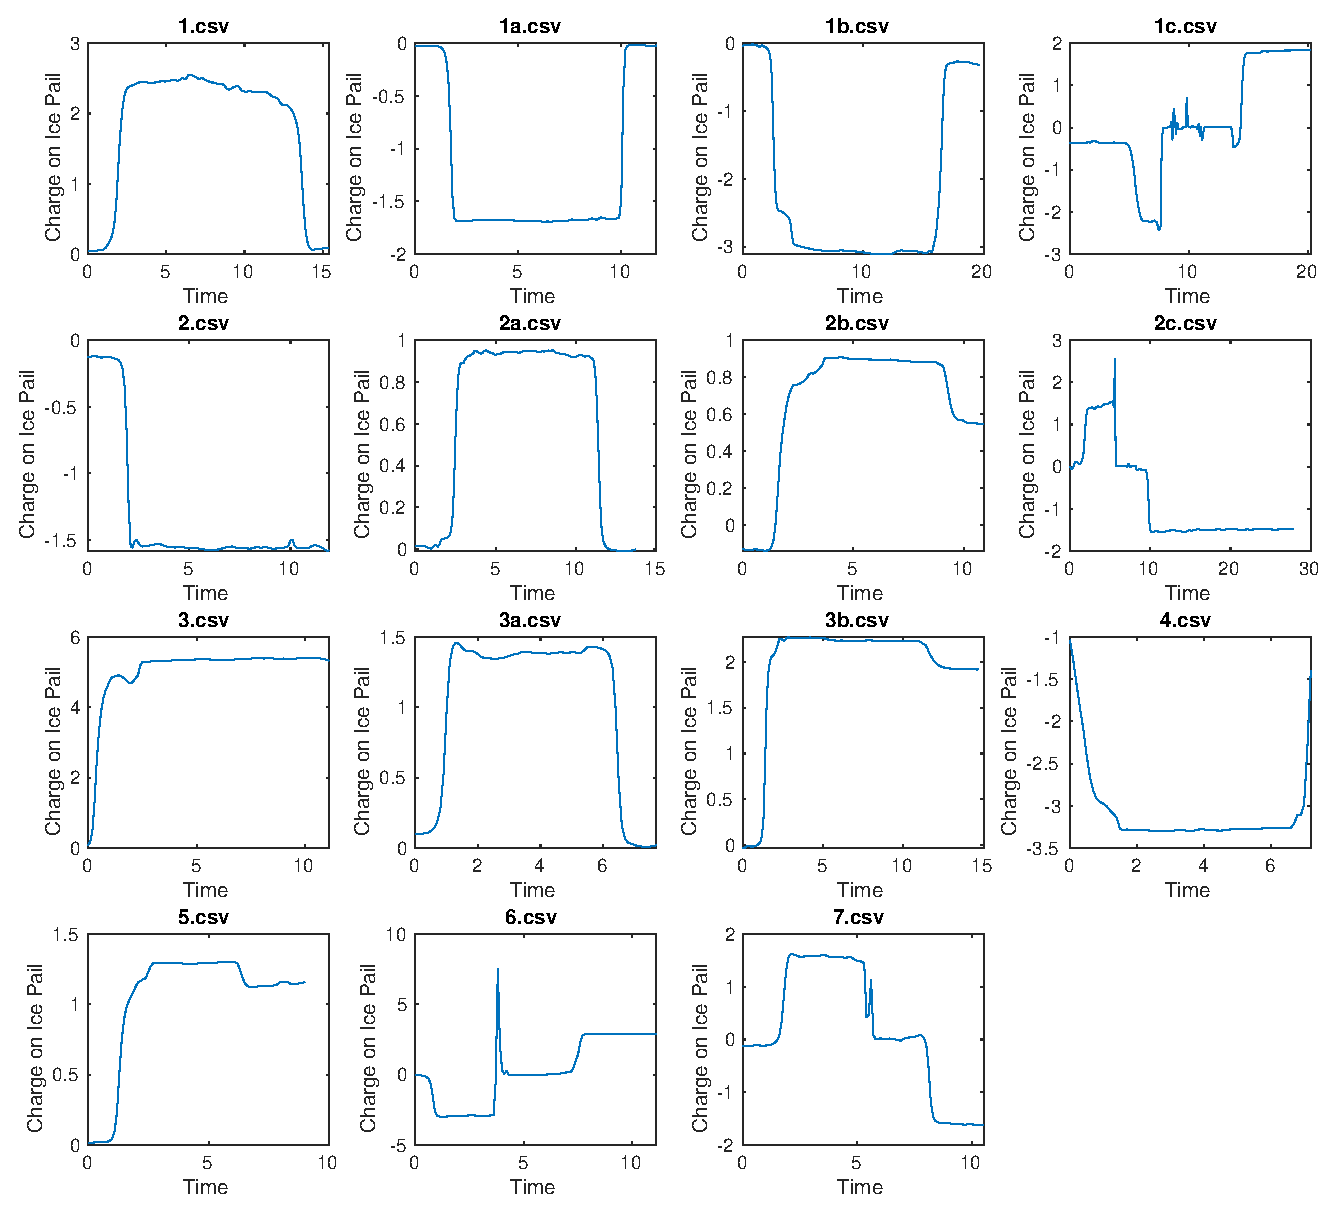
\includegraphics[width=0.8\textwidth]{figure1.eps}
\caption{All data we took for Experiment 1, without any data cleaning and choice of data set.}
\label{fig:exp1data}
\end{figure}



\subsection{Experiment Y: Name of Y} 
% Results and discussion for Experiment Y.

% Examples again.
\begin{figure}[H]
    \begin{subfigure}{0.5\textwidth}
\centering
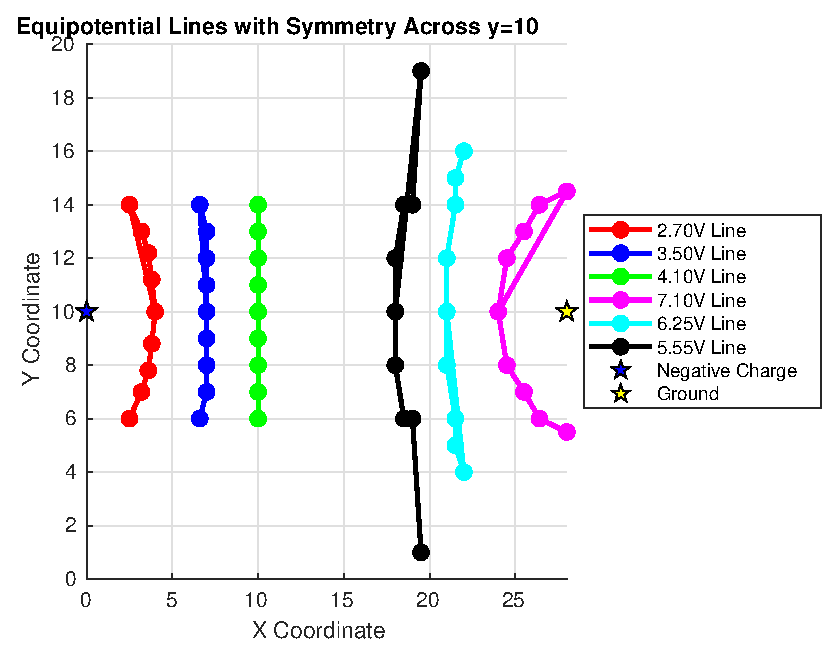
\includegraphics[width=0.8\textwidth]{EquipotentialLines.eps}
\caption{Drawn equipotential lines from MATLAB.}
\label{sfig:eq}
    \end{subfigure}
    \begin{subfigure}{0.5\textwidth}
\centering
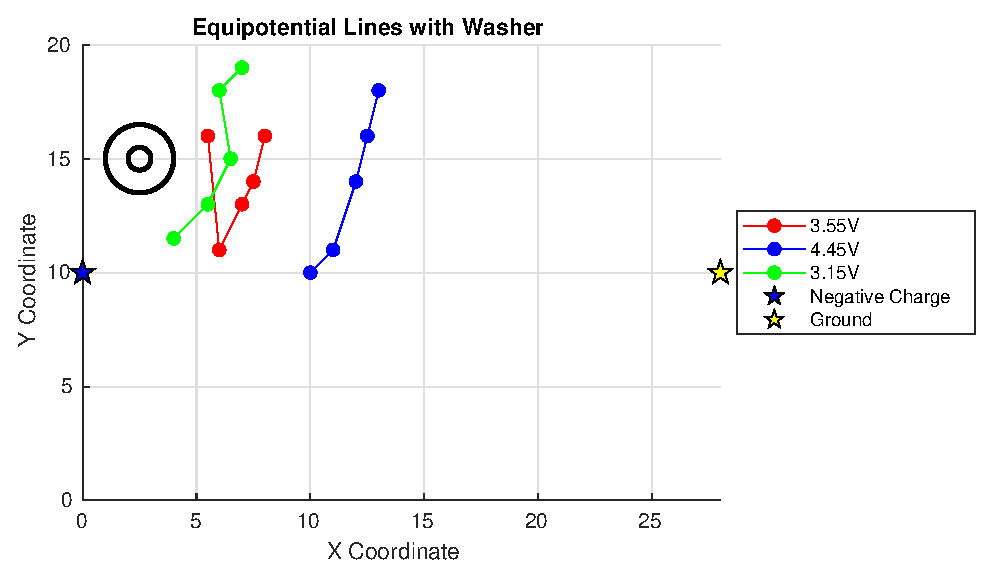
\includegraphics[width=1\textwidth]{EquipotentialLinesWithWasher.eps}
\caption{Drawn equipotential lines with washer on the paper from MATLAB.}
\label{sfig:eqwasher}
    \end{subfigure}
    \caption{Experiment results of Experiment 2 Part A and B.}
    \label{fig:exp2data}
\end{figure}


% Used this vspace command to reduce the distance between figures and the title, you can remove, comment or increase it as you wish.
\vspace{-1cm}
\section{Conclusions}
% Combined conclusions for both experiments.



\section{Names of the Participants}


% A simple table for participants and their contributions.
\begin{table}[H]
    \centering
    \begin{tabular}{| c : c |}
    \hline
        \textbf{Participants} & \textbf{Their Contribution} \\
    \hline\hline
        John Doe (writer of this report) & Contribution of YOURSELF. \\
    \hline
        John Smith & Contribution of John Smith \\
    \hline
    \end{tabular}
    \caption{Even though everyone focused on specific things, we mostly tried each others jobs too.}
\end{table}


% In case you need a special section for Extra Credit, uncomment below line and starting doing the magic.
% \section{Extra Credit}

\section{References}

% List of references in not-so-appropriate format, I was too lazy to use other packages. This does not give the output of APA 7th or latest APA; however, you can use other standards as you wish.
\bibliographystyle{apalike}
% To use all the cited sources, give intext citation as given example before, if you cannot do that but insist on adding those, uncomment below line. 
% \nocite{*}
\vspace{-1cm} % Reduce the distance between title and citations.
\bibliography{references} % No .bib extension

\section{Appendices}


% Add, remove, or change the order of the items as you wish.
\begin{enumerate}
    \item MATLAB Code
    \item Images
    \item Figures % I highly recommend adding figures to the Appendices section aswell.
\end{enumerate}

\subsection{1. MATLAB Code}
% Include MATLAB code snippets or link to repository.

% Examples of how to add MATLAB code as a listing.
\lstinputlisting[caption={MATLAB Code for Our Collective Plot of Data in Figure~\ref{fig:example}}, label={lst:collective_plot}]{Exp1PartA.m}
\vspace{10pt} % Adds some vertical space between the code block and the explanation

\lstinputlisting[caption={MATLAB Code for Equopotential Line Figure}, label={lst:collective_plot}]{Exp2PartA.m}
\vspace{10pt} % Adds some vertical space between the code block and the explanation

\lstinputlisting[caption={MATLAB Code for Equopotential Line with Washer Figure}, label={lst:collective_plot}]{Exp2PartB.m}
\vspace{10pt} % Adds some vertical space between the code block and the explanation

\subsection{2. Images}
% Include photographs, drawings, etc.
% The below command is quite buggy, it is recommended not to uncomment it.
% \setcounter{figure}{0}
% You can use figure environment to add images in a flexible way.


\subsection{3. Figures}
% Include figures
\setcounter{figure}{0}
\begin{figure}[H]
\centering
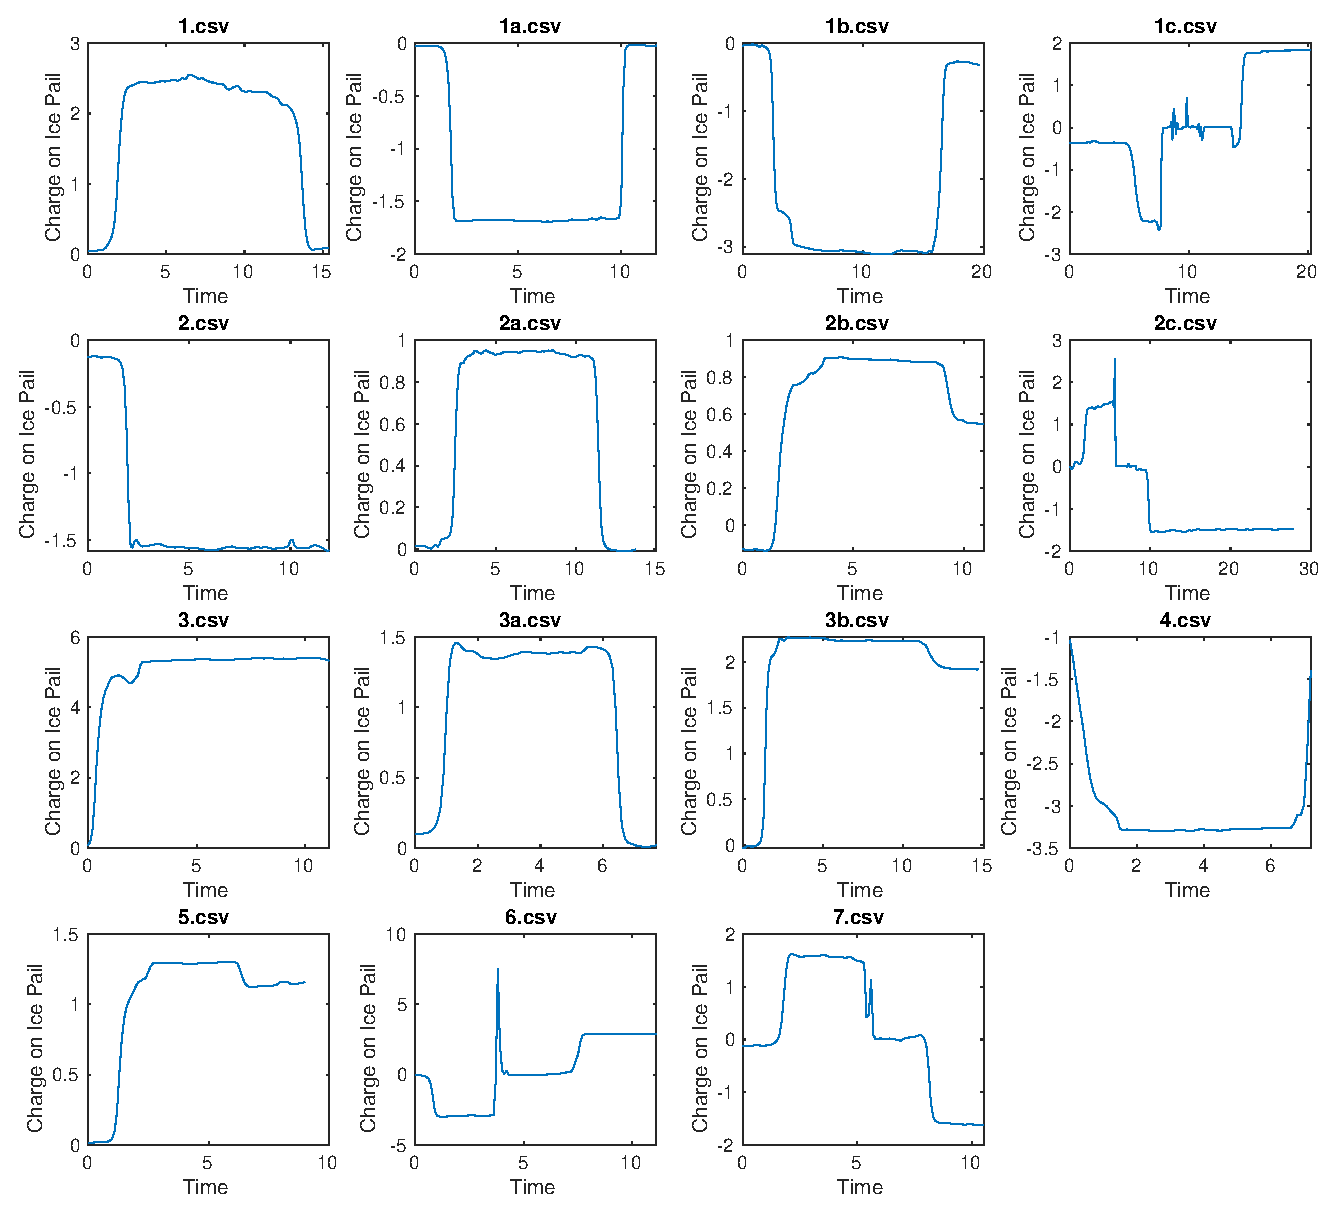
\includegraphics[width=0.8\textwidth]{figure1.eps}
\caption{All data we took for Experiment 1, without any data cleaning and choice of data set. Mentioned as Fig~\ref{fig:example}}
\end{figure}

\begin{figure}[H]
\centering
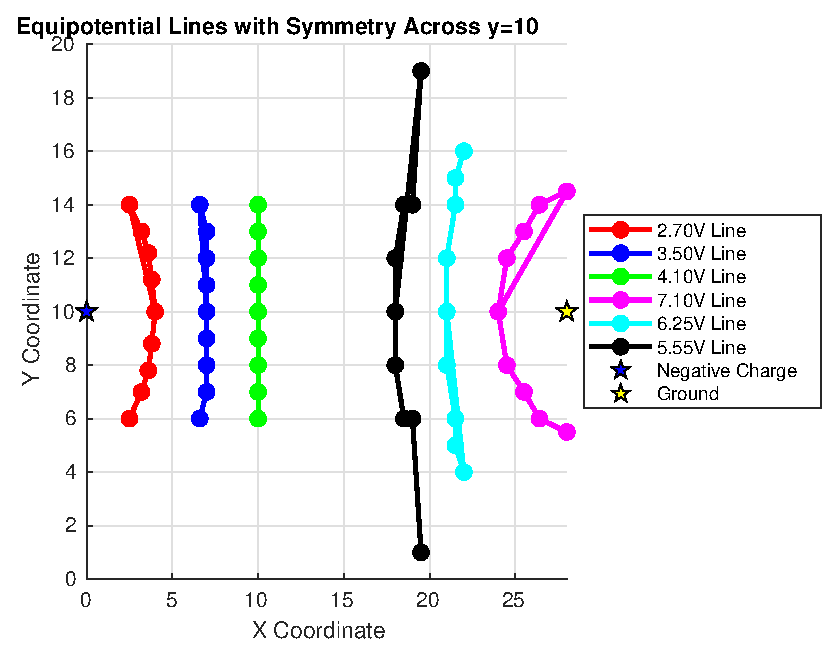
\includegraphics[width=0.8\textwidth]{EquipotentialLines.eps}
\caption{Drawn equipotential lines from MATLAB. Mentioned as Fig~\ref{fig:eq}}
\end{figure}

\begin{figure}[H]
\centering
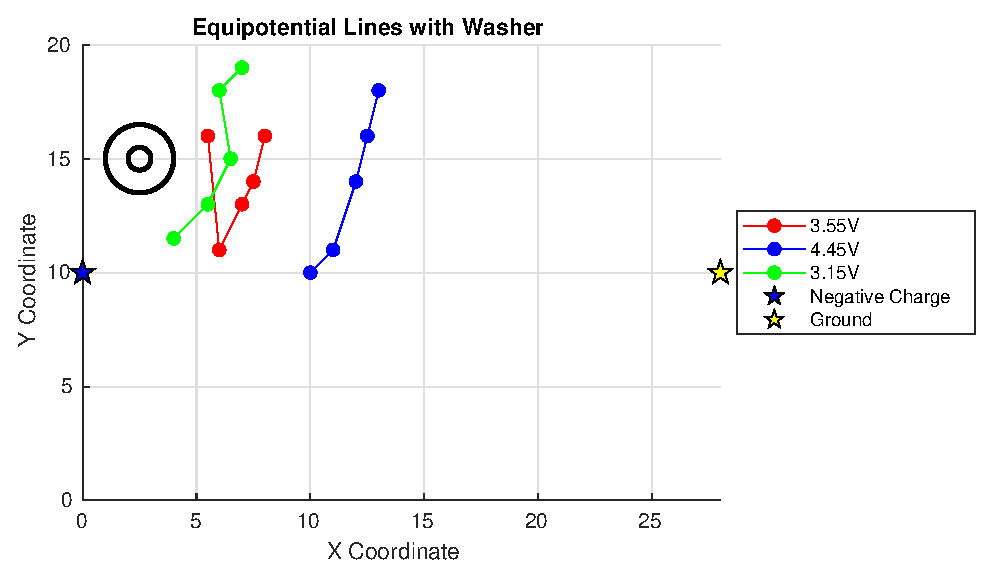
\includegraphics[width=0.8\textwidth]{EquipotentialLinesWithWasher.eps}
\caption{Drawn equipotential lines from MATLAB. Mentioned as Fig~\ref{fig:eqwasher}}
\end{figure}

\end{document}
